\section{Architecture Principles}
\label{sec:background}

%Prior to getting into the details of our algorithm,

We overview our design choices, as motivated by today's leading key-value store implementations.
We discuss their API, approaches to scaling them, and the LSM approach to data management.

\subsection{Data Model and API}
\label{ssec:kvs}

In key-value stores~\cite{Bigtable2006,PNUTS2008,hbase}, the data is comprised
of items ({\em rows}) identified by unique keys. A row value is a (sparse) bag of attributes called {\em columns}.
The internal structure of data items is largely opaque for the rest of our discussion.
%Co-accessed columns (typically used by the same application) can be aggregated
% in {\em column families} to optimize access.

The basic API of a key-value store includes \emph{put} and \emph{get} operations to store and retrieve values by their keys.
Updating an item is cast into putting an existing key with a new value, and deleting
one is performed by putting a \emph{deletion marker}, $\NULL$, as the key's value.

To cater to the demands of online analytics applications (e.g.,~\cite{Percolator2010}), key-value stores typically
support \emph{snapshot scans}, which provide consistent read-only views of the data. A scan allows the user to acquire a
snapshot of the data (\emph{getSnap}), from which the user can iterate over
items in lexicographical order of their keys by applying \emph{next} operations.

Geo-replication scenarios drive the need to reconcile conflicting replicas.
This is often done through vector clocks~\cite{Dynamo07}, which require the key-value store
to support conditional updates, namely, atomic read-modify-write
operations.

\subsection{Scalability in Distributed Key-Value Stores}
Distributed key-value stores achieve scalability by sharding data into units called {\em partitions}
(also referred to as \emph{tablets}~\cite{Bigtable2006, PNUTS2008} or \emph{regions}~\cite{hbase}).
%There is a variety of methods to shard data by
%key, range and hash partitioning being most notable~\cite{GrayTP1993}.
%
Partitioning provides {\em horizontal scalability} -- stretching the service across multiple servers.
%Production web-scale stores are comprised of thousands of such servers~\cite{Bigtable2006}, each managing
%dozens of partitions~\cite{hbaseRegionArch}.
Nevertheless, there are penalties associated with having many partitions, as argued in~\cite{hbaseRegionArch}:
First, the data store's consistent snapshot scans do not span multiple partitions. Analytics applications that
require large consistent scans are forced to use costly transactions across shards.
%Second, the system-level meta-data increases with the number of partitions, and can become a bottleneck.
%
Second, this requires a system-level mechanism for managing partitions~\cite{Bigtable2006,PNUTS2008,hbase}, whose meta-data size depends on the number of partitions, and can become a scalability bottleneck.




The complementary approach of
increasing the serving capacity of each individual partition is called
\emph{vertical scalability}. First, this necessitates optimizing the speed of I/O-bound operations.
The leading approach to do so, especially in write-intensive settings,
is  LSM  (discussed in Section~\ref{ssec:lsm}), which
%replaces random disk accesses with sequential I/O,
effectively eliminates the disk bottleneck.
Once this is achieved, the rate of in-memory operations becomes paramount (as we show in Section~\ref{sec:eval}).
Increasing this rate is the challenge we focus on in this paper.

We argue here that we can improve performance while reducing the number of partitions,
which in turn allows for larger snapshot scans and reduces meta-data size.
To illustrate this point, Figure~\ref{fig:production_partitions} shows sample results from our experiments (the experiment
setup is detailed in Section~\ref{sec:eval}). In this example, we evaluate {\clsm\/} with one big partition
versus {\leveldb\/} and {\hyperleveldb\/} with four small partitions, where each small partition's workload
is based on a distinct production log, and the big partition is the union thereof. Each of the small partitions is served
by a dedicated one quarter of the thread pool (resource separation), whereas the big partition is served by all
worker threads (resource sharing).
We see that {\clsm\/}'s improved concurrency control scales better than partitioning, achieving a peak throughput of above 1 million operations/sec -- approximately 25\% above the competition.


\begin{figure}[t]
\centerline{
{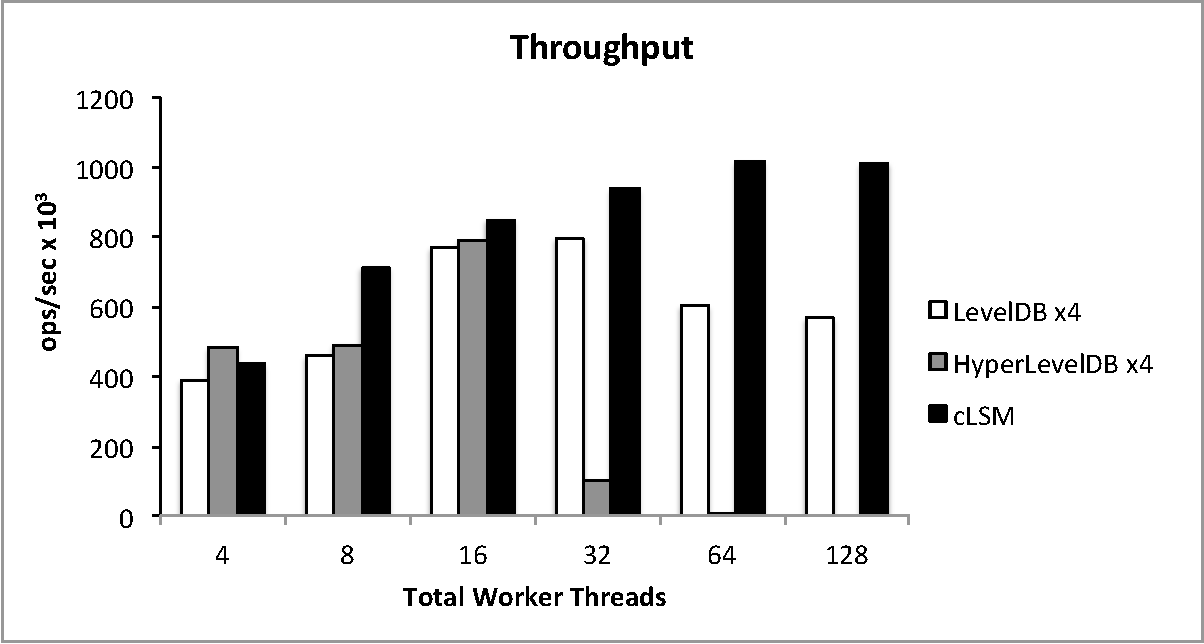
\includegraphics[width=\columnwidth]{Figures/prod4Partitions.pdf}}
}
\caption{\bf{Comparing two approaches to scalability with production workload.
The resource-isolated configuration exercises {\leveldb\/} and {\hyperleveldb\/} with
4 separate partitions, whereas the resource-shared configuration evaluates {\clsm\/} with
one big partition. }}
\label{fig:production_partitions}
\end{figure}


\remove{
One way to boost vertical scalability is keep partitions small, which reduces the need for concurrency control.
However, this approach also introduces new limitations. First, high partitioning granularity erodes the magnitude
of bulk disk operations performed by the LSM-DS merge function, thus adversely impacting the I/O
bottleneck~\cite{hbaseRegionArch}. In addition, it impedes sharing the server's resources (e.g., buffer
cache) across the partitions. We therefore strive to achieve vertical scalability by exploiting concurrency,
rather than by highly granular data partitioning.
}

\remove{
These phenomena are
manifested in the evaluation of our concurrent
algorithm over a complete instance of the database versus competitors that
utilize partitioning of the data (Section~\ref{sec:realworkloads}).
%Secondly, it puts the database's metadata service under strain.
%
On the semantic side, the atomicity of large scans across multiple partitions
(even on a single machine) can be addressed only via a
transactional processing layer~\cite{Percolator2010, Omid2014}, which is beyond
the scope of this work.
}

\subsection{Log-Structured Merge}
\label{ssec:lsm}

Disk access is a principal bottleneck in storage systems,
and remains a bottleneck even with today's
SSDs~\cite{Tanenbaum:2014:MOS,RocksDBBenchmarks,Wu:2012:AWB}. Since reads are often effectively masked by
caching, significant emphasis is placed on improving write throughput and latency~\cite{Tanenbaum:2014:MOS}.
It is therefore not surprising that log-structured merge solutions~\cite{O'Neil1996}, which batch writes  in memory
and merge them with on-disk storage in the background, have become the de facto
choice for today's leading key-value stores~\cite{Bigtable2006, FBMessaging2012, leveldb, RocksDB, Hyperdex2012, BLSM2012}.

An LSM data store organizes data in a series of components of increasing sizes, as illustrated in Figure~\ref{fig:tri}.
The first component, $C_m$, is an in-memory sorted
map that contains most recent data. The rest of the
components $C_1, \ldots, C_n$ reside on disk. For simplicity, in the context of
this work, they are perceived as a single
component, $C_d$.
An additional  important building block is the
\emph{merge} procedure, (sometimes called \emph{compaction}), which incorporates the contents of the memory component
into the disk, and the contents of each component into the next one.



\remove{
The choice of $C_m$'s size is affected by the merge procedure's performance.
On the one hand, $C_m$ should not be too big, to allow the merge to complete
fast and release the buffer for future use. On the other hand, it should not be too
small, to avoid frequent read/write spikes that access the same data many times
and waste the potential of sequential I/O~\cite{hbaseRegionArch}.
}


\remove{
In order to differentiate the interface of the internal map data structure from
that of the entire LSM-DS, we refer to the corresponding functions of the in-memory data structure
as \scode{insert} and \scode{find}.
%More precisely, the in-memory data structure supports at least the following two operations:
\begin{description}
\item [\scode{insert(k,v)}] -- inserts the key-value pair $(k,v)$ into the map.
If $k$  exists, the value associated with it is over-written.
A key is removed by inserting a $\NULL$ value.
\item[\scode{find(k)}] -- returns a value $v$ such that
 the map contains an item $(k,v)$, or $\NULL$ if no such value exists.
\end{description}
}

A put operation inserts an item into the main memory
component $C_m$, and logs it in a sequential file for recovery
purposes. Logging can be configured to be synchronous (blocking) or asynchronous
(non-blocking). The common default is asynchronous logging, which avoids waiting
for disk access, at the risk of losing some recent writes in case of a crash.

When $C_m$ reaches its size limit, which can be hard or soft, it is merged with
component $C_d$, in a way reminiscent of merge sort: The items of both $C_{m}$ and $C_{d}$, %or sub-ranges thereof,
are scanned and merged. %in memory buffers.
The new merged component
is then migrated to disk in bulk fashion, replacing the old component.
When considering multiple
disk components, $C_m$ is merged with component $C_1$.
Similarly, once a disk component $C_{i}$ becomes full its data is migrated to the
next component $C_{i+1}$.
Component merges are
%often referred to as \emph{compaction}, and are performed as
%background processes.
%Size management is done in a wrapper of the in-memory component, with a simple counter
%increment and check. Size limit can be hard or soft.
%
%The merge function is executed in a series of steps -- each step spans a key
% range.
%It is
executed in the background as an automatic maintenance service.


The get operation may require going
through multiple components until the key is found. But when get operations are
applied mostly to recently inserted keys, the search is completed in $C_m$.
Moreover, the disk component utilizes a large RAM cache. Thus, in workloads
that exhibit locality, most requests that do access  $C_{d}$ are satisfied from RAM
as well.

During a merge, the memory component becomes immutable,
at which point it is denoted
as $C'_m$. To allow put operations to be executed while rolling the merge, a
 new memory component $C_m$ then becomes available for updates (see
Figure~\ref{fig:comp}).
The put and get operations access the
components through three global pointers: pointers $P_m$ and $P'_m$ to the
\emph{current} (mutable) and \emph{previous} (immutable) memory components, and
pointer $P_d$ to the disk component. When the merge is complete, the previous
memory component is discarded. Allowing multiple puts and gets to be executed
in parallel is discussed in the sequel.

\begin{figure*}
  \centering
  \begin{subfigure}[t]{0.43\textwidth}
   \center
{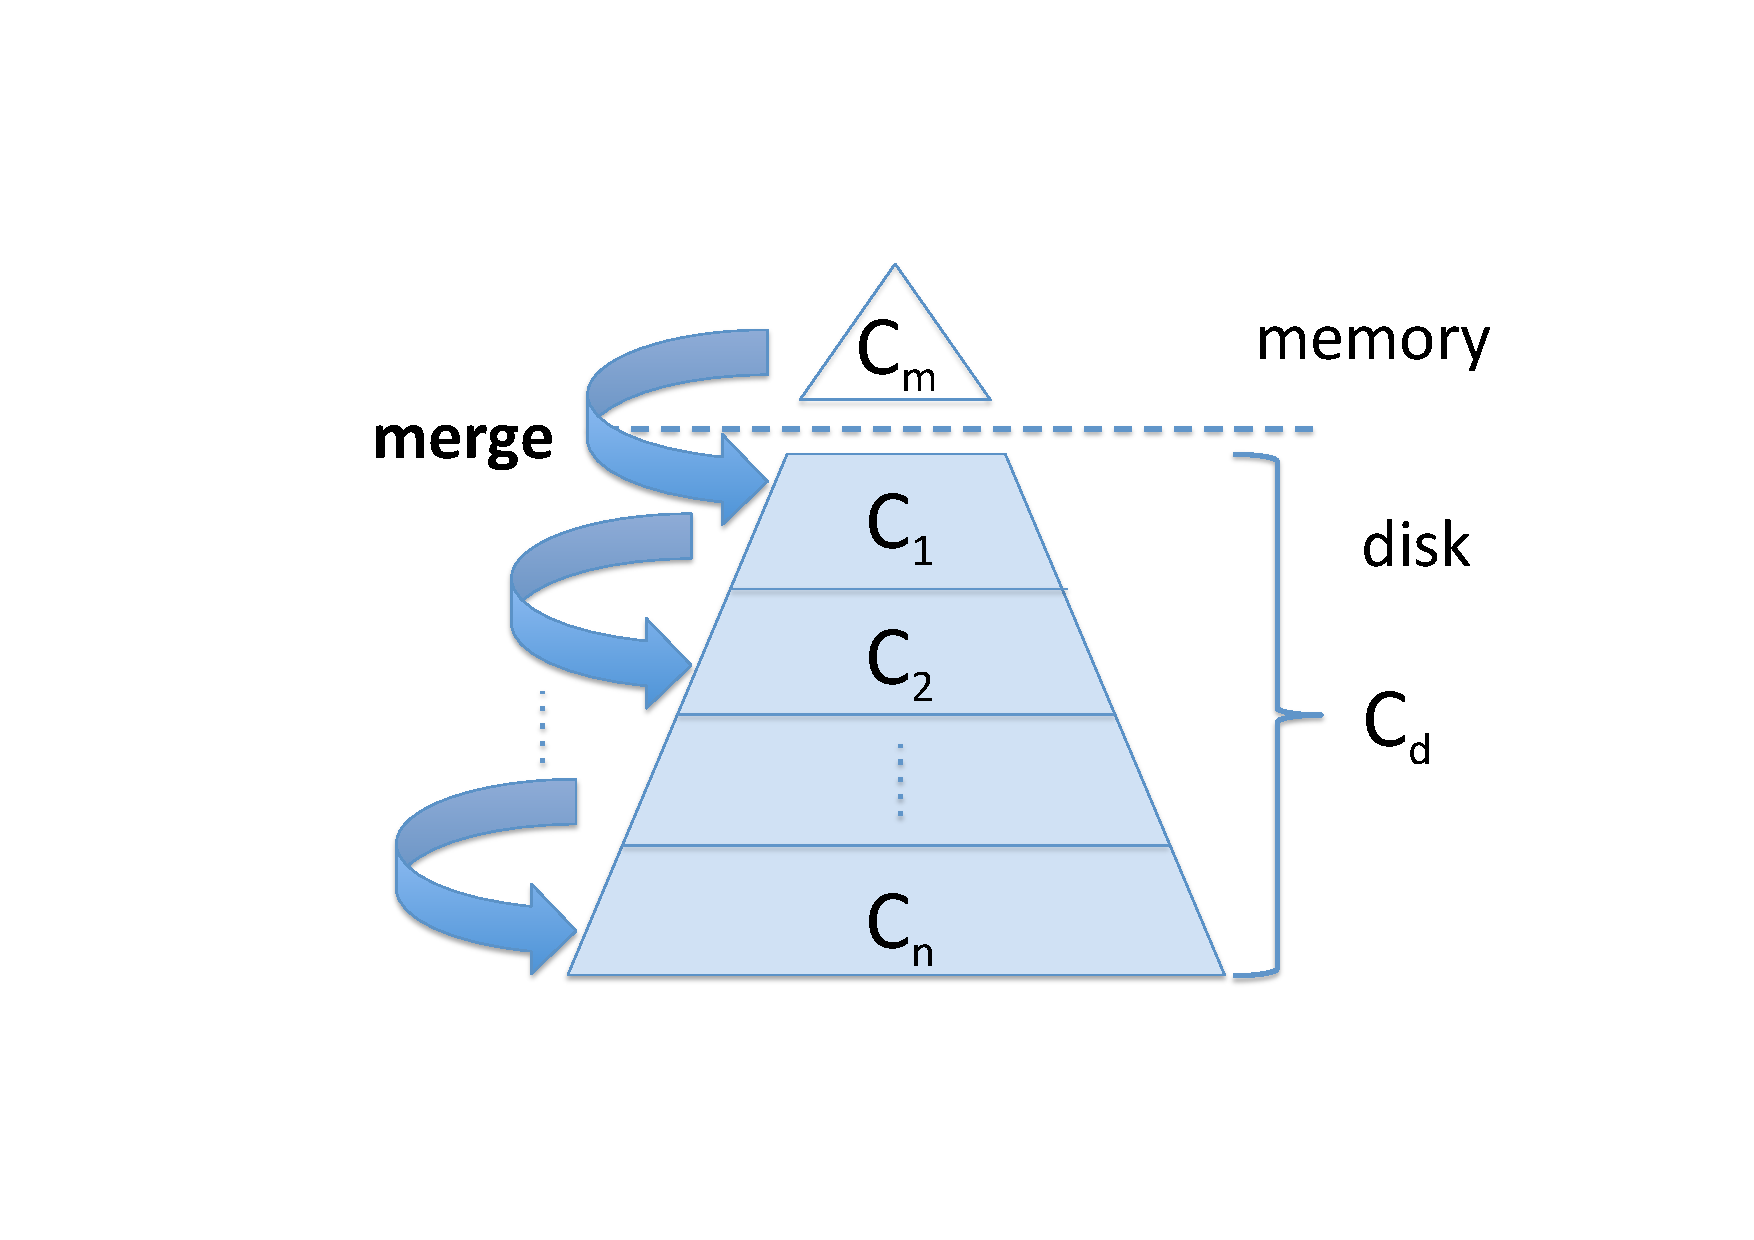
\includegraphics[width=0.6\textwidth,clip, trim =180 100 125 130]{Figures/triangle.pdf}} \caption{LSM-DS consists of a small memory component, and a large disk component
 comprised of a series of components of increasing sizes.}
               \label{fig:tri}
  \end{subfigure}%
  \hspace{0.1\textwidth}
  \begin{subfigure}[t]{0.43\textwidth}
   \center
{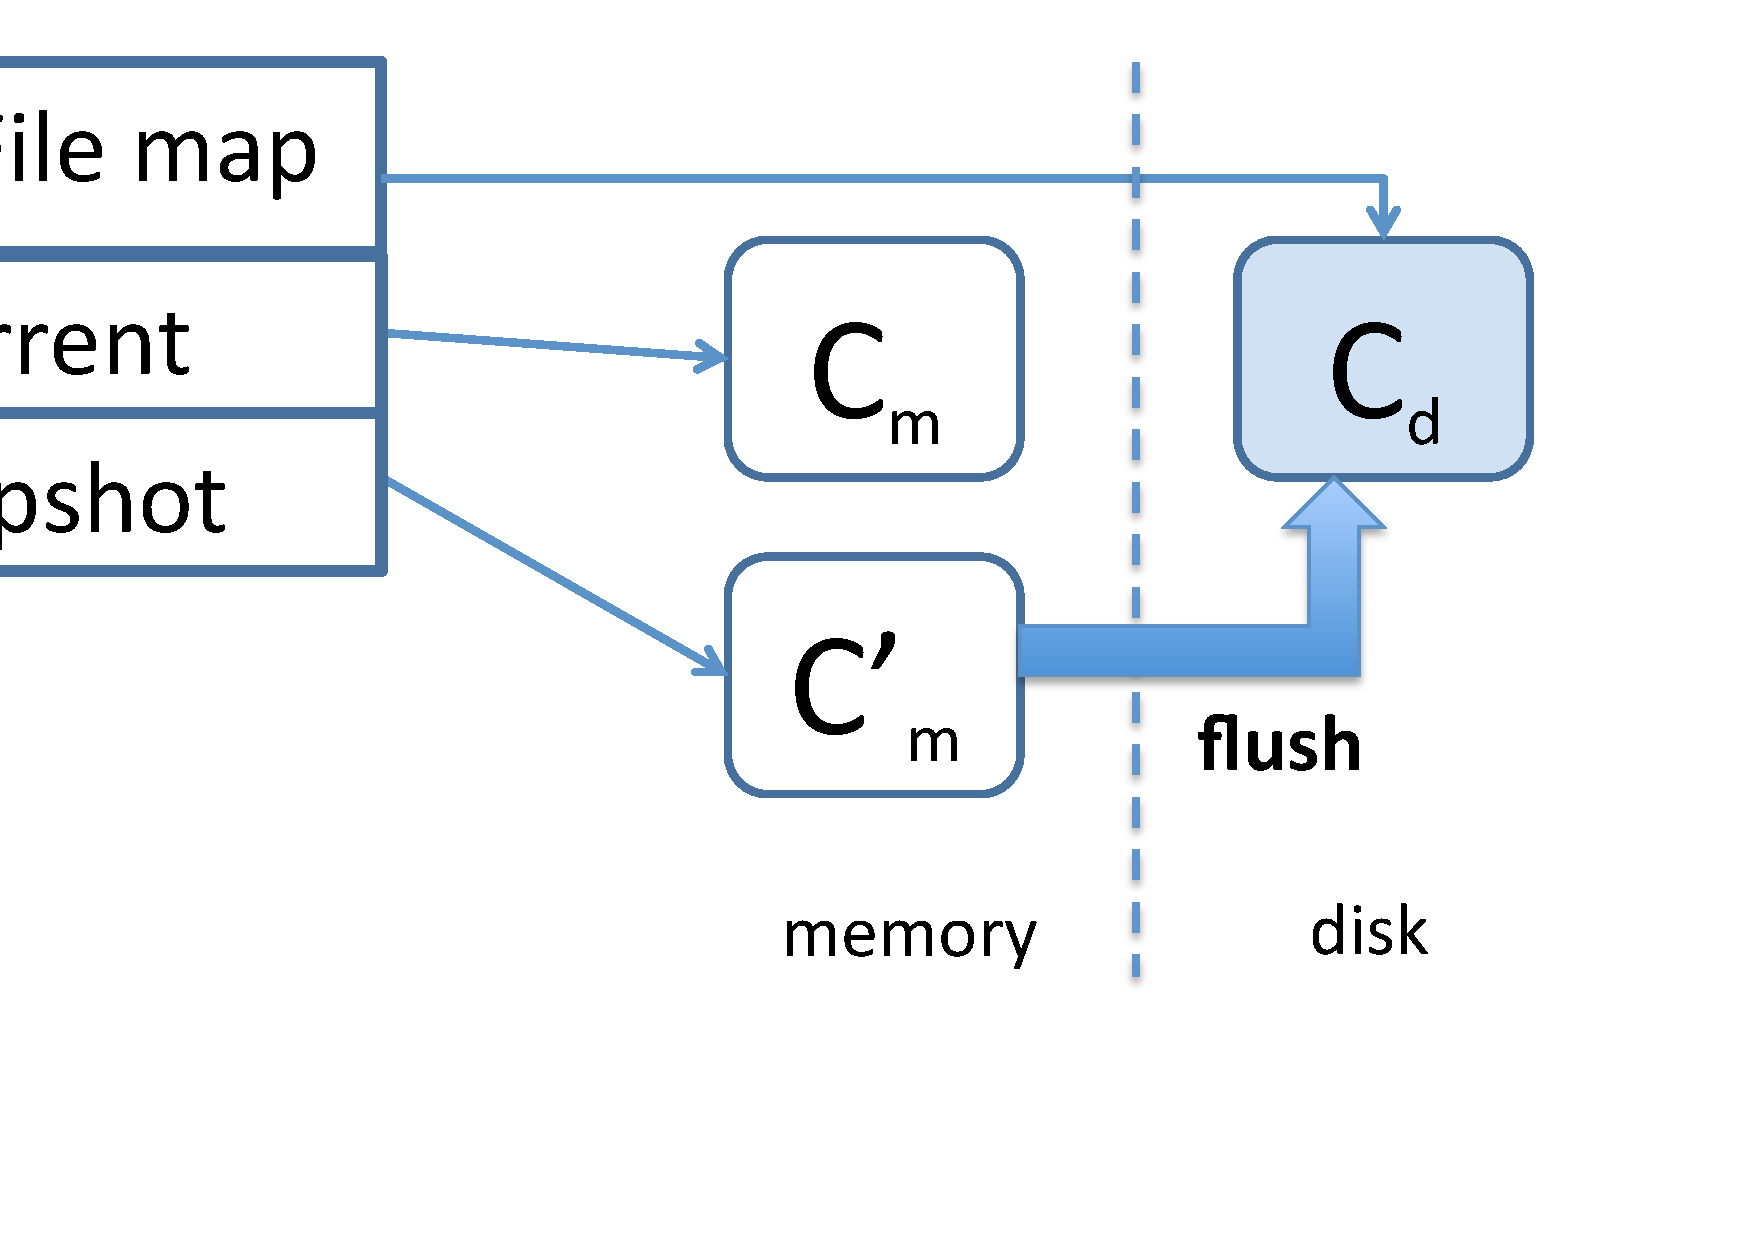
\includegraphics[width=0.6\textwidth,clip, trim =40 100 100 25]{Figures/architecture.pdf}} \caption{Global pointers $P_m$ to current (mutable) memory component
$C_m$, $P'_m$ to previous (immutable) memory component $C_m^{'}$, and $P_d$ to
disk component $C_d$. Merge incorporates  $C_m^{'}$ into $C_d$, while new
items are added to $C_m$.}
               \label{fig:comp}
  \end{subfigure}%
  \caption{\bf LSM-DS architecture.}
\label{fig:architecture}
\end{figure*} 